\documentclass[12pt]{article}
\usepackage[english]{babel}
\usepackage[margin=0.80in]{geometry}
\usepackage{amsmath}
\usepackage{amssymb}
\usepackage[mathcal]{euscript}
%\usepackage{urwchancal}
\usepackage{algorithm}
\usepackage[noend]{algpseudocode}
\usepackage[utf8]{inputenc}
\usepackage{graphicx}
\usepackage{listings}
\usepackage{color}
\usepackage{hyperref}
\usepackage{cite}
\numberwithin{figure}{section}
\numberwithin{table}{section}

\definecolor{mygreen}{rgb}{0,0.6,0}
\definecolor{mymauve}{rgb}{0.58,0,0.82}
\definecolor{mygray}{rgb}{0.97,0.97,0.97}
  
\lstset{
  language=C++,
  basicstyle=\footnotesize,
  commentstyle=\color{mygreen},
  keywordstyle=\color{blue},
  stringstyle=\color{mymauve},
  tabsize=4
}

\begin{document}
\begin{titlepage}
\title{Project 4 - FYS4150}
\author{Jostein Brændshøi}
\date{
    Department of Physics\\%
    University of Oslo\\[2ex]%
    \today
}
\clearpage
\maketitle
\thispagestyle{empty}

\begin{abstract}
\noindent We study the evolution of thermal energy and spin interactions in a magnetic material using the 2D Ising model and Monte Carlo simulations. We implement a parallel Ising model and look statistical properties of the system for various lattice sizes and number of Monte Carlo cycles. We find that the convergence towards the most likely state (and the most likely state itself) depends strongly on temperature in correspondence with the underlying Boltzmann distribution. We also find that different initial spin configurations improves or worsen the convergence. Finally we look at phase transitions and see that the Ising model gives rise to second order phase transitions that are more pronounced for larger lattice sizes. Also the associated critical temperature is found to be in fairly good agreement with Lars Onsager (1944) exact results \cite{LarsOnsager}.
\end{abstract}
\vspace{2.00cm}

\noindent The address \url{https://github.com/jostbr/FYS4150-Projects/tree/master/Project4} on Git-Hub is associated with this project. Here one can find all code used in the project. This includes C++ source files containing the core of the project, but also Python plotting scripts for result visualization. There are also available benchmark results from running the code as well as \LaTeX \ source for this PDF. The parameters behind the benchmark simulation results are described throughout this report. Also, if one wishes closer plot inspection, running the Python visualization script reproduces all plots in this report directly using the data files in the benchmark directory.

\end{titlepage}
\pagebreak

% ======== Indicate new section
% -------- Indicate new subsection

% ========================================================================================
% ========================================================================================
\section{Introduction} \label{sec:intro}
The use of statistics in science is a continuously growing area and make huge impacts in a range of fields. Stochastic methods are becoming increasingly popular and especially as powerful computers are more and more easily accessible (even as laptops in many cases), the potential for such methods continue to grow. Monte Carlo methods are even the methods of choice in many areas of physics, like for example statistical physics and in particular solid state physics. Hence, gaining experience with Monte Carlo methods may be very valuable for a physicist. This brings us to the contents of this project.
\vspace{0.30cm}

\noindent In this project we will employ methods in statistical physics and implement the binary 2D Ising model in order to simulate spin interactions in e.g. a solid metal. In this model each spin in the material can only take on two directions, either $+1$ or $-1$, hence it is a binary model. Working with the Ising model, we study the response of a magnetic material to thermal energy. In particular, we look at the evolution of the magnetic spin configuration in the material that undergoes neighbouring spin interactions as response to thermal energy. As is a very popular use of the Ising model, we will apply it to see if we can identify phase tranbsitions \cite{Comp}.
\vspace{0.30cm}

\noindent Specifically, the structure of this report involves firstly discussing some analytical results that will help us greatly when implementing the Ising model. Then we move on to some technicalities about the model before describing the verification process undergone to make sure the model behaves as it should. Mentions on code performance improvements (parallelization) are discussed. Then we discuss results with a main focus on the evolution of various statistical expectation values for the system and attempt to apply some of the underlying physics of the Ising model in order to 


%====================================================================================
%====================================================================================
\section{Theory}
As an initial exercise it is useful to look at some analytical results for a small sample size lattice of, say, $2\times2$. The usefulness in this exercise is mainly to have results to which we can compare the later obtained numerical solutions, but such an exercise also serves as a stepping stone into working with and understanding the Ising model. We consider a $2\times2$ lattice, meaning a total of four spins, and assume that each spin can only take on the two possible values $\pm 1$, i.e. a binary system as mentioned in section \ref{sec:intro}. We also use boundary boundary conditions giving the condition that the neighbour of an edge spin is at the opposite side of the lattice. We want to compute the partition function $Z$, expectation values of the energy $E$ and absolute value magnetic moment $|\mathcal{M}|$, the specific heat $C_v$ and the magnetic susceptibility $\chi$.
\vspace{0.30cm}

\noindent Before we can obtain the expression for any of the mentioned quantities we have to find the energy and magnetic moment of each of the $M$ possible spin configurations offered by the $2\times2$ lattice. Due to it being four spins each with two possible values ($\pm 1$) for the spin, we have a total of $M=2^4=16$ different possible spin configurations in the lattice. From \cite{Comp} and \cite{pro4} we have the Ising model formula for computing the energy of configuration $i$ by
\begin{equation}
	E_i=-\mathcal{J}\sum_{\langle kl \rangle}s_k^is_l^i \label{eq:E}
\end{equation}
where $s_k$ is the spin value of the $k$'th spin, $\langle kl \rangle$ indicates a double sum, but only over nearest neighbours (i.e. e.g. for each $k$, $l$ loops over the nearest neighbours of $k$) and $\mathcal{J}$ is a constant describing the strength of the interaction between neighbouring spins in the lattice. Computing the total magnetic moment of the lattice is a more straight-forward operation where we simply sum up all spin values according to \cite{Comp}
\begin{equation}
	\mathcal{M}_i=\sum_{i=j}^Ns_j^i \label{eq:M}
\end{equation}
Applying \eqref{eq:E} and \eqref{eq:M} to the $2\times2$ lattice with periodic boundary conditions, we get
\begin{align}
	E_i&=s_1^is_2^i+s_1^is_3^i+s_2^is_1^i+s_2^is_4^i+s_3^is_4^i+s_3^is_1^i+s_4^is_3^i+s_4^is_2^i \label{eq:E_2x2}\\
	\mathcal{M}_i&=s_1^i+s_2^i+s_3^i+s_4^i \label{eq:M_2x2}
\end{align}
where in the nearest neighbour sum (for energy) we have only counted each neighbour spin product once (they appear twice due to periodic boundary conditions). If one were to draw out all 16 spin configurations, one would see that one could group the configurations into categories as displayed in table \ref{tab:2x2}. In this table, \eqref{eq:E_2x2} and \eqref{eq:M_2x2} have been used for each of the $M=16$ configurations. As can be seen, many of the configurations are duplicates of each other, e.g. the case with one spin equal to $+1$ and the other three equal to $-1$ gives four possible positions to find the $+1$ value, but they all produce the same energy and magnetic moment. This particular case corresponds with row 5 in the table.
\vspace{0.30cm}

\begin{table}[ht]
\begin{center}
  \begin{tabular}{| c | c | c | c |}
  	\hline
  	Spins $=+1$ & Duplicates & Energy & Moment \\[0.05cm] \hline\hline
     4 & 1 & $-8\mathcal{J}$ & 4\\[0.10cm]
     3 & 4 & $0$ & 4\\[0.10cm]
     2 & 4 & $0$ & 0\\[0.10cm]
     2 & 2 & $+8\mathcal{J}$ & 0\\[0.10cm]
     1 & 4 & $0$ & -2\\[0.10cm]
     0 & 1 & $-8\mathcal{J}$ & -4\\[0.10cm]
     \hline
  \end{tabular}
\end{center}
\caption{The energy and magnetic moment for all $M=16$ spin configurations in a $2\times2$ lattice.}
\label{tab:2x2}
\end{table}

\noindent We are now in a position where we can move on to find the quantities initially mentioned in this (SUB)section. The Ising model is based on the Boltzmann distribution \cite{Comp}
\begin{equation}
	P'(\beta)=e^{-\beta E} \label{eq:boltzmann_dist}
\end{equation}
where the marked $P$ indicates a non-normilized distribution and $\beta=1/k_BT$ inversely proportional with the temperature $T$ of the system under study, i.e. the lattice, and $k_B$ is the Boltzmann kosntant. Firstly we compute the partition function for the distribution (for normalization of the distribution) by summing over all spin configurations \cite{Comp}
\begin{equation}
	Z=\sum_{i=1}^MP_i'(\beta)=\sum_{i=1}^Me^{-\beta E_i}=2e^{8\beta\mathcal{J}}+2e^{-8\beta\mathcal{J}}+12=4\cosh(8\beta\mathcal{J})+12 \label{eq:Z_2x2}
\end{equation}
Then we find the expectation values of the energy and magnetization as well as their square expectation values through the standard statistical expressions by summing over spin configurations and using the values in table \ref{tab:2x2}:
\begin{align}
	\langle E \rangle&=\frac{1}{Z}\sum_{i=1}^ME_ie^{-\beta E_i}=-\frac{32\mathcal{J}\sinh(8\beta\mathcal{J})}{Z} \label{eq:E_2x2_avg}\\[0.20cm]
	\langle E^2 \rangle&=\frac{1}{Z}\sum_{i=1}^ME_i^2e^{-\beta E_i}=\frac{256\mathcal{J}^2\sinh(8\beta\mathcal{J})}{Z} \label{eq:E2_2x2_avg}\\[0.20cm]
	\langle |\mathcal{M}| \rangle&=\frac{1}{Z}\sum_{i=1}^M|\mathcal{M}_i|e^{-\beta E_i}=\frac{1}{Z}(8e^{8\beta\mathcal{J}}+16) \label{eq:M_2x2_avg}\\[0.20cm]
	\langle |\mathcal{M}|^2 \rangle&=\frac{1}{Z}\sum_{i=1}^M|\mathcal{M}_i|^2e^{-\beta E_i}=\frac{32}{Z}(e^{8\beta\mathcal{J}}+1) \label{eq:M2_2x2_avg}
\end{align}
which further allows us to compute the heat capacity $C_v$ (at constant volume) through \cite{Comp}
\begin{equation}
	C_v=\frac{1}{k_BT^2}\left(\langle E^2 \rangle-\langle E \rangle^2\right)=-\frac{1}{k_BT^2Z}\left\{256\mathcal{J}^2\cosh(8\beta\mathcal{J})-\frac{\left[32\mathcal{J}\sinh(8\beta\mathcal{J})\right]^2}{Z}\right\} \label{eq:Cv_2x2}
\end{equation}
and the magnetic susceptibility $\mathcal{X}$ as \cite{Comp}
\begin{equation}
	\chi=\frac{1}{k_BT}\left(\langle |\mathcal{M}|^2 \rangle-\langle |\mathcal{M}| \rangle^2\right)=-\frac{1}{k_BTZ}\left[32(e^{32\beta\mathcal{J}}+1)-\frac{(8e^{8\beta\mathcal{J}}+16)^2}{Z}\right] \label{eq:X_2x2}
\end{equation}
It's worth remembering that all these quantities are functions of the temperature $T$ through $\beta=1/k_BT$. We now have some analytical results for the $2\times2$ lattice case and this will serve as useful comparison and validation material for the implementation of the Ising model below.


% ========================================================================================
% ========================================================================================
\section{Methods}

%-----------------------------------------------------------------------------------
%-----------------------------------------------------------------------------------
\subsection{Ising model}
The methods used in this project are mainly related to the Ising model and the Metropolis algorithm\cite{Comp}. We use stochastic methods, in particular Monte Carlo methods, in order to simulate the spin interactions in a 2D lattice as a response to the thermal energy of the system. the main idea with the method is that we start the lattice in some spin configuration (every spin is either $+1$ or $-1$), and then we start flipping spins and have a sophisticated rule for what spin flips to accept in order to go to a new spin configuration. Then we calculate the energy and magnetic moment for the new configuration and update the expectation values for these quantities. Then we repeat this for a large number of Monte Carlo cycles in order to obtain decent statistics. The above mentioned sophisticated rule is the Metropolis algorithm and defines the sampling rule for accepting a move to a new spin configuration. The code on GitHub is an implementation of the algorithm described in pseudo code on page 435 in \cite{Comp}. It is attempted to have frequent comments in the code and more about the Ising model and Metropolis algorithm can be seen from there.

%-----------------------------------------------------------------------------------
%-----------------------------------------------------------------------------------
\subsection{Model verification/testing}
To make sure an implementation of a numerical model is reasonable, it is invaluable and very useful to have analytical results to which one can compare the numerical ones. Here, we are in a position where we have known analytical expressions, in the $2\times2$ lattice, for quantities of interest in equations \eqref{eq:E_2x2_avg} through \eqref{eq:X_2x2}. One might argue that the discussion in this particular subsection also could have been grouped together with the other results below in section \ref{sec:results}, but primary use of the $2\times2$ case was under development and verification of the model. It lays the foundation before one could, with confidence, extend the simulations to the larger lattices where analytical expressions are harder to come by. Therefore the author decides it fits slightly better here.
\vspace{0.30cm}

\noindent One can view Table \ref{tab:2x2_model_verification} as a summary of the verification tests of the implementation of the Ising model. Here we compute analytical values for the expectation value of the energy $\langle E \rangle$ and absolute magnetization $\langle |M| \rangle$ as well as heat capacity $C_v$ and magnetic susceptibility $\chi$, all using the equations \eqref{eq:E_2x2_avg} through \eqref{eq:X_2x2}. These are then the values to which we compare the numerical results produced by the model for various choices of the total number of Monte Carlo cycles/sweeps.

\begin{table}[ht]
\begin{center}
\def\arraystretch{1.5}
  \begin{tabular}{| c | c | c | c | c | c | c |}
  	\hline
  	& MC cycles & $\langle E \rangle$ & $\langle |M| \rangle$ & $C_v$ & $\chi$ & Exec time [s]\\[0.05cm] \hline\hline
  	Numerical & $10^2$ & -1.98000 & 0.995000 & 0.1584000 & 0.00990000 & 0.00025 \\[0.05cm] \hline
  	Numerical & $10^3$ & -1.98200 & 0.993500 & 0.1427040 & 0.02083100 & 0.00055 \\[0.05cm] \hline
  	Numerical & $10^4$ & -1.99100 & 0.997150 & 0.0716760 & 0.00806751 & 0.00240 \\[0.05cm] \hline
  	Numerical & $10^5$ & -1.99558 & 0.998460 & 0.0352819 & 0.00481051 & 0.03709 \\[0.05cm] \hline
  	Numerical & $10^6$ & -1.99614 & 0.998701 & 0.0308204 & 0.00393026 & 0.14306 \\[0.05cm] \hline
  	Numerical & $10^7$ & -1.99595 & 0.998651 & 0.0323185 & 0.00404142 & 1.37764 \\[0.05cm] \hline
  	Numerical & $10^8$ & -1.99596 & 0.998656 & 0.0322280 & 0.00401855 & 7.65786 \\[0.05cm] \hline
  	Numerical & $10^9$ & -1.99598 & 0.998660 & 0.0320946 & 0.00401503 & 69.3750 \\[0.05cm] \hline
  	Analytical & N/A & -1.99598 & 0.998661 & 0.0320787 & 0.00401074 & N/A \\[0.05cm] \hline
  \end{tabular}
\end{center}
\caption{Comparing numerical and analytical results for $\langle E \rangle$, $\langle |M| \rangle$, $C_v$ and $\chi$ int the $2\times2$ lattice case with temperature $T=1.0$ J and $\mathcal{J}=k_B=1$. Also the lattice was initialized with a random spin configuration. Note that all values are "per-spin" (divided by total number of spins (4 in this case)). Numerical results are computed by 4 parallel MPI processes as well as compiled with optimization flags.}
\label{tab:2x2_model_verification}
\end{table}

\noindent One can see that there are fairly good correspondence between the numerical and analytical values for $\langle E \rangle$ and $\langle |M| \rangle$ already at very low number of Monte Carlo cycles for this $2\times2$ case. However the heat capacity and susceptibility are not satisfactory in agreement with their analytical counterparts this early on. When we reach around $10^6$ Monte Carlo cycles, all four quantities seem to be within acceptable limits. Although, what's acceptable here can be very subjective, but at least for $10^6$ cycles, all quantities are within 96\% of the analytical value. However, if one is only interested in the mean energy and mean magnetization, far fewer cycles are needed to achieve good agreement.

%-----------------------------------------------------------------------------------
%-----------------------------------------------------------------------------------
\subsection{Parallelization}
The computations in this project use a lot of CPU time due to the vast number of Monte Carlo cycles we perform, and thus, emphasis has been put on the speed of the program. In particular, the computationally heavy nature of the project motivates implementation of parallel execution of the code. To achieve this the Message-Passing-Interface (MPI) \cite{MPI} has been used. The workings of the Monte Carlo simulations in the Ising model makes parallelization quite accessible. The main idea is that divide the total number of Monte Carlo cycles we wish to run between all the MPI process ad let each run its own set of Monte Carlo cycles and locally keep track of the computations of the expectation values. Then when we e.g. wish to write out the expectation values to file (or the simulation is done. i.e. each process is done with their Monte Carlo cycles) we sum up all local expectation values from each MPI process and collect the total expectation values at the master process. In practice this operation is done by using the \texttt{MPI\_Reduce()} function. See next section for performance gains resulting from utilising the discussed parallelization.

%-----------------------------------------------------------------------------------
%-----------------------------------------------------------------------------------
\subsection{Timing}
Here we will briefly discuss the time gains made by two performance enhancements done to the code. One of the being the parallelization discussed in the above subsection and the other being use of optimization compiler flags for the C++ compiler in order to enable features such as vectorization of loops. Standard compiled C++ programs does not have optimization features turned on and creates a full size direct translation of the C++ code into machine code. This means the program will not run as fast as it potentially can with enabled optimization flags for the compiler. Indeed this was experienced during running of the simulations in this project and a speedup of a factor 10 was achieved using optimization flags and vectorization. This saved significant amounts of time. In addition we have the speedup we gain from parallelizing the code as described above. The laptop used for running the simulations described in this report had 4 available CPU cores. Thus the logical choice for number of MPI processes to use, was 4. Observing execution times of a simulation with $10^6$ Monte Carlo cycles for a $20\times20$ lattice gave an average of 25 seconds with 1 process while 4 MPI processes gave an average of 7.5 seconds execution time, yielding a speedup of 3.3. While we would expect to get a speedup closer to 4, this is almost impossible due to the fact that when you add MPI there are also associated startup costs for the processes as well as time used in communication between the processes (although there isn't that much inter-process communication in this project, only one reduce call). There is no point in trying to run on more than 4 processes in this case as then MPI would just spawn virtual more virtual processe per CPU core which would instead slow down the program (due to more overhead) instead of giving additional speedup.
\vspace{0.30cm}

\noindent To summarize, combining the speedup from optimization flags and parallelizing with MPI gave a speedup of roughly factor 33 compared to the original non-vectorized serial code. Some additional timing data can be seen in the rightmost column in table \ref{tab:2x2_model_verification}. Here it appears that the execution time scales  linearly with number of Monte Carlo cycles, which is intuitively reasonable. However the execution time scales much worse with the lattice size considering the double loop over the lattice.

% ========================================================================================
% ========================================================================================
\section{Results} \label{sec:results}
We now move to look at some results from running the Ising model for various lattice sizes and. Key features we will be looking at include equilibration time, i.e. how many Monte Carlo cycles are required before the system reaches its most likely state, state acceptance dependence on temperature, probability distribution for the Ising model energy, signs of phase transitions and closer looks at the critical temperature.

%-----------------------------------------------------------------------------------
%-----------------------------------------------------------------------------------
\subsection{Reaching the most likely state} \label{sec:most_likely_state}
Let us look a $20\times20$ lattice and study the amount of Monte Carlo simulations needed in order to reach the most likely state. We set up a simulation using $L=20$ spins in each direction and a total of $10^8$ Monte Carlo cycles. We perform the computations both for $T=1.0$ J and for $T=2.4$ J. We repeat this for both an ordered (all spins pointing up) and random initial initial spin configuration. We are interested in looking at the development of the mean energy $\langle E \rangle$ and mean magnetization $\langle |M| \rangle$ as functions of number of Monte Carlo cycles. The results from the simulations are visualized in figure \ref{fig:20x20_EM}. The plots are zoomed in on to get a better impression of the convergence towards the equilibrium state (the initial values for $\langle E \rangle$ and $\langle |M| \rangle$ are far outside the scope of the $y$-axis in the plots, but showing these initial values would make everything else look flat).

\begin{figure}[ht]
 \centerline{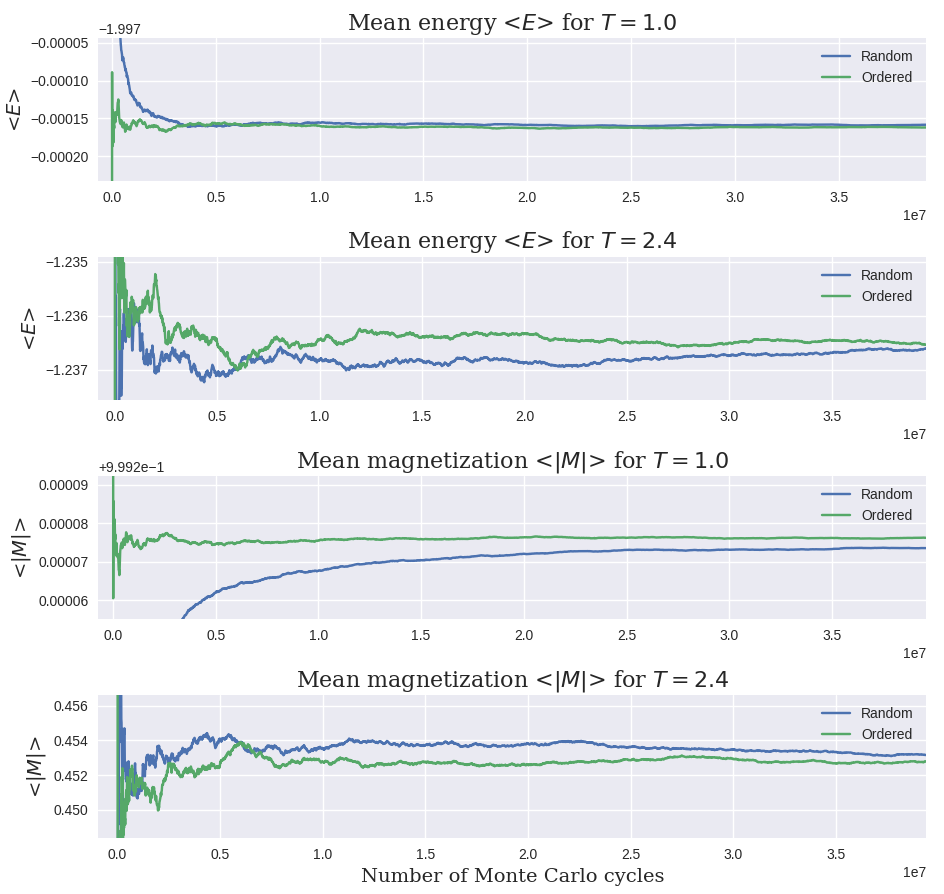
\includegraphics[scale = 0.60]{20x20_EM}}
 \caption{Results for the $20\times20$ lattice for mean energy $\langle E \rangle$ and mean magnetization $\langle |M| \rangle$ as a function of number of Monte Carlo cycles. Simulations are done for both a temperature $T=1.0$ J and for $T=2.4$ J and with $10^8$ Monte Carlo cycles for each temperature.}
 \label{fig:20x20_EM}
\end{figure}

\noindent Firstly, we may look note from figure \ref{fig:20x20_EM} that both the mean energy and mean magnetization move towards what looks like equilibrium states, for both temperatures and for both initial spin configurations. This is promising and reasonable based on the workings of the Metropolis sampling algorithm, but what are the number of cycles needed before the most likely state is reached and what are the factors that impact it? Looking at the graph we may read values of Monte Carlo cycles in the range $[1.1\cdot10^6, 5.0\cdot10^6]$ for all four panels in the figure. There is, though, significant differences for the initial spin configurations within each of the temperature runs. In particular, for the $T=1.0$ case, the most likely state is reached a lot quicker (both for $\langle E\rangle$ and $\langle |M| \rangle$) starting with an ordered configuration versus the random configuration. Especially the mean magnetization uses noteworthy more "time". A reason behind this could be related to the fact that when starting in an ordered configuration (all spins up) we have the minimum energy in the system in accordance with equation \eqref{eq:E} and as illustrated in table \ref{tab:2x2} for the $2\times2$ case. And for the lower $T=1.0$ of the two temperatures, this minimum energy would be closer to the most likely state (lower temperatures having lower energy in the most likely state. This can be seen in equation \eqref{eq:E_2x2_avg} for the energy expectation value using the Boltzmann distribution. A lower temperature gives a smaller exponent and thus smaller overall expectation value. We also see this on the $y$-axis in the plots) than for the upper $T=2.4$. This argument is also help explain why the ordered initial configuration does not appear that beneficial in the $T=2.4$ case. Here the random one even seem to be slightly better, although both are quite similar and produce about the same equilibration time.

\vspace{0.30cm}
\noindent Next we may note that for $T=2.4$, the system in general uses more time towards the most likely state, there are significantly larger oscillations (see scale of $y$.axis for the two temperature cases) about the most likely state. This can also be linked to the Boltzmann distribution and the Metropolis algorithm itself: In the Metropolis algorithm we have two options to accept a new configuration; either if the computed energy difference $\Delta E$ from the previous configuration is less than or equal to zero, i.e. $\Delta E\leq 0$, or if a random number $r\in[0,1]$ satisfies
\begin{equation}
	r\leq e^{-\beta\Delta E}=e^{-\Delta E/T} \label{eq:rleqw}
\end{equation}
with $\beta=1/T$ in our case (scaled temperature $k_BT\rightarrow T$). We can then see that if $T$ is larger (as in e.g. 2.4 versus 1.0), we get a larger exponent in \eqref{eq:rleqw} and thus a higher chance for $r$ to actually be smaller than $e^{-\Delta E/T}$ which further implies a higher chance for the system to accept the new configuration. In summary, and in other words, this reflects systems of higher temperatures having more "available" configurations/states to "jump" in and out of. This also seem reasonable with physical intuition and seems to be the reason behind the less "ordered" move towards the most likely state for the $T=2.4$ case.
\vspace{0.30cm}

\begin{figure}[ht]
 \centerline{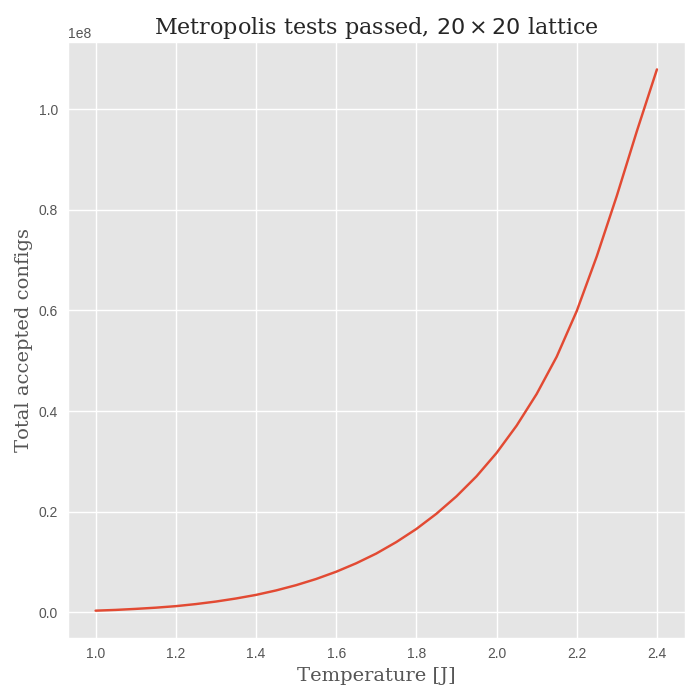
\includegraphics[scale = 0.60]{20x20_accepted_configs}}
 \caption{Plot showing the total number of accepted states (at total number of Monte Carlo cycles ($10^6$ for this plot)) as a function of temperature $T$ (with units energy due to scaling). For this figure, a random starting configuration was used for all temperatures.}
 \label{fig:20x20_AC}
\end{figure}

\noindent Another manifestation of this effect can be seen in figure \ref{fig:20x20_AC}. Here the $20\times20$ lattice simulation is run over a range of $T\in[1.0,2.4]$ with a temperature step $\Delta T=0.05$ and $10^6$ Monte Carlo cycles for each temperature. What's plotted is the total number of accepted configurations (at total Monte Carlo cycles) as a function of temperature. As the title suggest, this corresponds to plotting the number of passed Metropolis tests as a function of temperature. We observe that the number of accepted states exhibits an exponential-like behaviour on $T$. This brings us back to the above discussed specifics of the Metropolis test and the Boltzmann distribution. As $T$ increases the system becomes exponentially more prone to accept the new suggested configuration. This provides us with a link between figure \ref{fig:20x20_EM} and figure \ref{fig:20x20_AC}.


%-----------------------------------------------------------------------------------
%-----------------------------------------------------------------------------------
\subsection{Probability distribution}
In light of the all above talk about most likely states etc., we now move on to looking at the likelihood function for the energy, i.e. the probability distribution $P(E)$ for the energy in the $20\times20$ case. We are interested in seeing how the probability of the system is distributed (hopefully) around the expectation values discussed in the above section. To compute the distribution we count the occurrences of energies after each sweep through the lattice. However as the energy of the initial spin configuration is generally not very close to the most likely state, the move towards the most likely state would somewhat disturb our computations of the probability distribution. Thus we start counting the energy occurrences after we we have reached the most likely state. The chosen value for this is based on the discussion in section \ref{sec:most_likely_state}. To be well within limits of when the most likely state is reached, we choose to start the distribution counting after $6\cdot10^6$ Monte Carlo cycles. Then we count store the each energy for the next million Monte Carlo cycles and create a histogram of the distribution of the energy when oscillation about the most likely state.

\begin{figure}[ht]
 \centerline{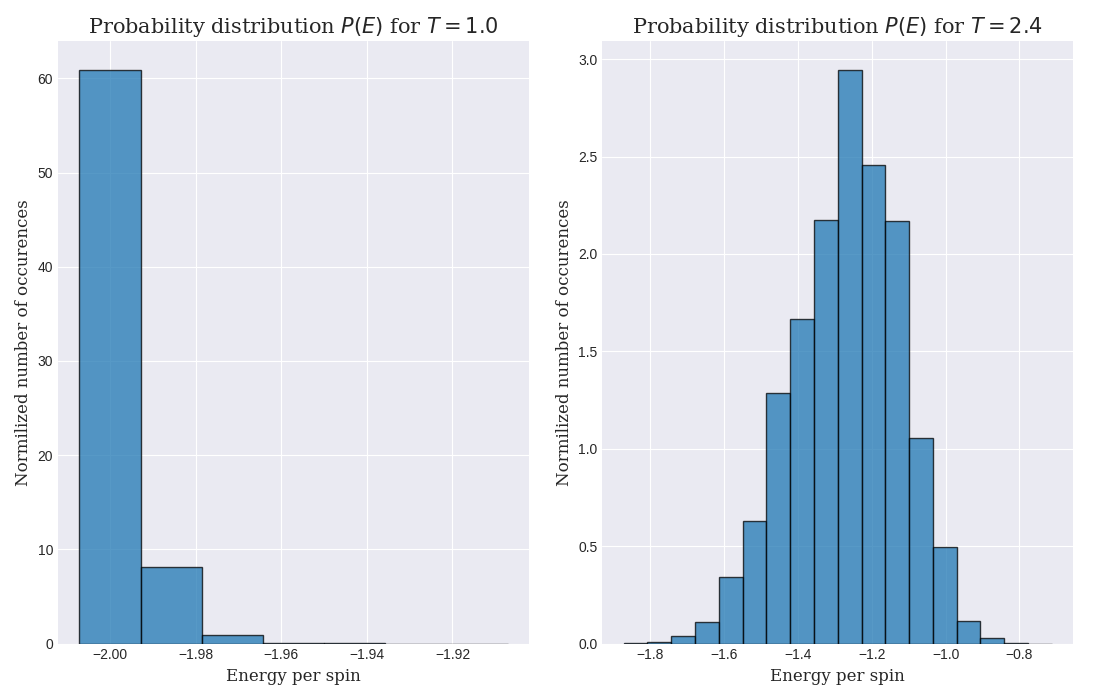
\includegraphics[scale = 0.60]{20x20_energy_dist}}
 \caption{Computed energy distribution $P(E)$ for the $20\times$ lattice at temperatures $T=1.0$ and $T=2.4$ by counting number of times various energies occur in the simulation. The counting was initiated after $6\cdot10^6$ cycles and $10^6$ sequential energy values were counted. A random initial configuration was used in both cases.}
 \label{fig:20x20_ED}
\end{figure}

\noindent This approach is done both for $T=1.0$ and for $T=2.4$ and the results can be seen in figure \ref{fig:20x20_ED}. Note that this histogram is normalized such that the area under the distributions integrate to 1. First of all we observe that peak of the distribution (for both temperatures) correspond well with the expectation values illustrated in figure \ref{fig:20x20_EM}. Next we observe a significant difference in the spread of the distributions. The spread is roughly one order of magnitude larger for the $T=2.4$ case. This is consistent with the discussion in section \ref{sec:most_likely_state} and again reflecting the larger tendency of accessing more states at higher temperatures in correspondence with the Boltzmann distribution behind the Ising model. Conversely for the lower temperature case, the system rarely jumps out of the ground state (all spins up) and almost all energy counts are for this energy. For further studying the spread, the variance $\sigma_E^2$ was calculated for the two simulations. For $T=1.0$, the variance was 0.027 which by visual inspection of the left panel in figure \ref{fig:20x20_ED} seems to correspond pretty well. However for the $T=2.4$ simulation, the variance was found to be $8.12$ which is a lot more than what the right panel in figure \ref{fig:20x20_ED} suggests. This caused confusion and one might have thought that the reason behind the anomaly was related to the fact that we compute the variance from the very start of the simulation and that the initial move towards the most likely state disturbed the value significantly. This was checked in the form of basing the variance computations only in the same Monte Carlo cycle interval $[6\cdot10^6,7\cdot10^7]$ as the distribution counting. This resulted in a variance of 8.06. Although slightly smaller than 8.12, the author concludes that the initial move towards the most likely state did not significantly disturb the proper value for the variance, and thus, the reason behind the discrepancy remains unclear.


%-----------------------------------------------------------------------------------
%-----------------------------------------------------------------------------------
\subsection{Phase transitions} \label{sec:phase_transitions}
Next we wish to see if we can identify a phase transition using the Ising model. In accordance with \cite{Comp}, the Ising model is expected to exhibit second order phase transitions. Our quest in this subsection is to try and identify them in our simulations. Our setup for this exercise is as suggested \cite{pro4}, i.e. we run simulations for lattices of sizes $40\times40$, $60\times60$ and $80\times80$. Unfortunately, due to long computation time for the $100\times100$ lattice, there was not enough time to include the results for this particular case. However we add the $20\times20$ lattice instead. For each of the lattices we simulate over a temperature range $T\in[2.2,2.34]$ (presumably close around the critical temperature for phase transitions) with a step of $\Delta T=0.02$ and use $4\cdot10^6$ Monte Carlo cycles (based on the equilibration times discussed in section \ref{sec:most_likely_state}. However, this is probably a bit too few cycles for the larger lattices here and the author wishes there were time for simulations with more Monte Carlo cycles) and compute the expectation values for the energy $\langle E \rangle$ and magnetization $\langle |M| \rangle$ as well as the specific heat $C_v$ and magnetic susceptibility $\chi$. Recall that the two latter quantities are calculated with the left formula in equations \eqref{eq:Cv_2x2} and \eqref{eq:X_2x2} after the simulation for each temperature.

\begin{figure}[ht]
 \centerline{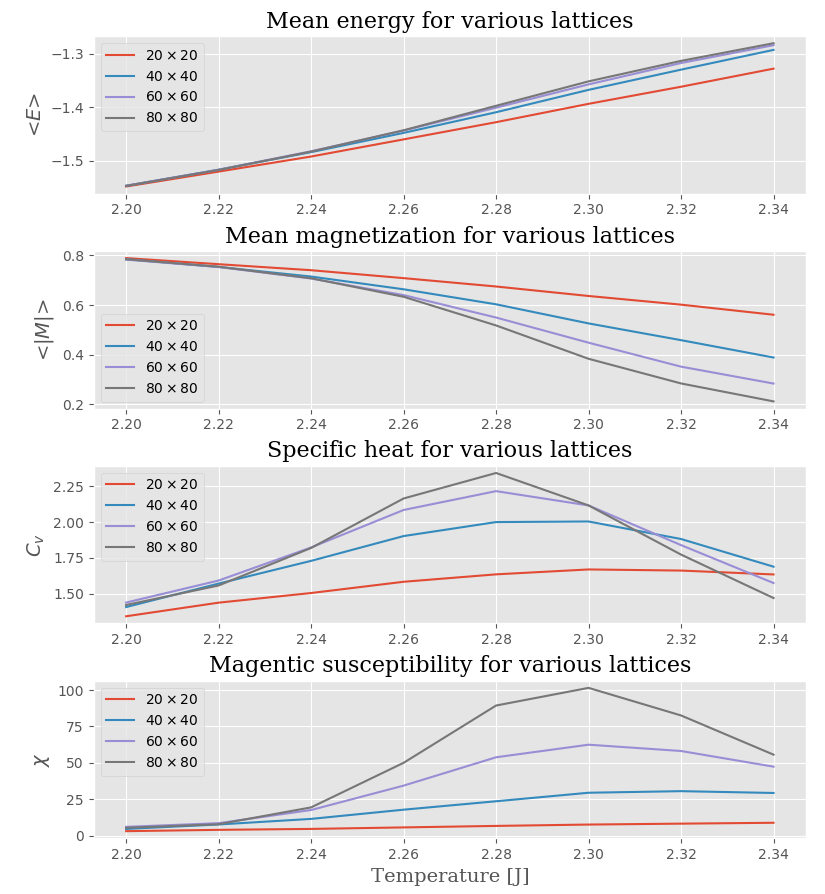
\includegraphics[scale = 0.62]{phase_transitions}}
 \caption{Computations of mean energy $\langle E \rangle$ and mean magnetization $\langle |M| \rangle$ as well as the specific heat $C_v$ and magnetic susceptibility $\chi$ in simulations for $T\in[2.2,2.34]$ with a step of $\Delta T=0.02$ and $4\cdot10^6$ Monte Carlo cycles. All repeated for 4 different lattice sizes.}
 \label{fig:phase_transition}
\end{figure}

\noindent In figure \ref{fig:phase_transition} we can see how the four mentioned quantities evolve as functions of temperature for each of the simulated lattices. In accordance with \cite{Comp} we have that, at the critical temperature the magnetic susceptibility will diverge. However in our case we have a finite sized lattice and are not in the thermodynamic limit where the lattice size $L\to\infty$. Thus we rather expect to find a large maxima in the susceptibility. Indeed this is what we see in the bottom panel in figure \ref{fig:phase_transition}. And so it seems like we are able to identify the signs of a phase transition. Also noteworthy is that this effect becomes more prominent for the larger lattices, i.e. the lattices further towards the thermodynamic limit where the diverging susceptibility takes place. In that sense the difference in the graphs for the various lattice sizes seem reasonable.

%-----------------------------------------------------------------------------------
%-----------------------------------------------------------------------------------
\subsection{Critical temperature}
How does the critical temperatures at which the phase transitions seem to occur in \ref{fig:phase_transition} compare with Lars Onsager exact results from 1944 \cite{LarsOnsager}? In order to answer this we utilize equation (3) in \cite{pro4}, which relates the critical temperature $T_C(L)$ for a finite lattice of size $L\times L$ with the corresponding one for an infinitely large lattice $T_C(L=\infty)$ i.e.
\begin{equation}
	T_C(L)-T_C(L=\infty)=aL^{-1/\nu} \label{eq:T_C_infinite}
\end{equation}
where $a$ is a constant and the exponent constant $\nu$ that in accordance with \cite{Comp} and \cite{pro4} have an exact value of $\nu=1$. Applying \eqref{eq:T_C_infinite} for two lattices with sizes $L_1\times L_1$ and $L_2\times L_2$ gives us the opportunity to write
\begin{align*}
	T_C(L_1)-T_C(L=\infty)&=\frac{a}{L_1} \\[0.20cm]
	T_C(L_2)-T_C(L=\infty)&=\frac{a}{L_2}
\end{align*}
and solving this set of equations for $T_C(L=\infty)$ by eliminating $a$ gives
\begin{equation}
	T_C(L=\infty)=\frac{L_2T_C(L_2)-L_1T_C(L_1)}{L_2-L_1} \label{eq:compare_onsager}
\end{equation}
Reading the critical temperature at the susceptibility maxima in figure \ref{fig:phase_transition} lets us then use \eqref{eq:compare_onsager} to compare our simulation results with the exact value found by Onsager. First we list the values we read for $\chi$ maxima in figure \ref{fig:phase_transition}. These values can be seen in table \ref{tab:critic_temps}

\begin{table}[ht]
\begin{center}
\def\arraystretch{1.5}
  \begin{tabular}{| c | c | c | c | c |}
  	\hline
  	$L$ & 20 & 40 & 60 & 80 \\[0.05cm] \hline
  	$T_C(L)$ [J] & 2.34 & 2.32 & 2.30 & 2.30 \\[0.05cm] \hline
  \end{tabular}
\end{center}
\caption{Values of critical temperature (units energy) read of from the magnetic susceptibility (bottom panel) in figure \ref{fig:phase_transition}.}
\label{tab:critic_temps}
\end{table}

\noindent Using for instance the critical temperatures for $L_1=80$ and $L_2=40$ and inserting into \eqref{eq:compare_onsager} gives $T_C(L=\infty)=2.28$ Joules which corresponds fairly well with Onsagers exact result of $2/\ln(1+\sqrt{2})\approx 2.269$ \cite{LarsOnsager}. Similar numbers can be found by using other combinations of $L_1$ and $L_2$ from table \ref{tab:critic_temps}. It's worth noting that, as can be seen in table \ref{tab:critic_temps} and figure \ref{fig:phase_transition}, the critical temperature identified for $L=80$ is the one that itself is closest to the exact result, further reinforcing the reasoning from section \ref{sec:phase_transitions} that the larger lattices will better approximate the results for the thermodynamic limit $L\to\infty$ This is also intuitively reasonable.
\vspace{0.30cm}

\noindent Areas for improvement in the above calculations include the fairly moderate amount of Monte Carlo cycles used and the resolution in temperature. In order to gain higher accuracy we would have like to have used even more cycles and a smaller temperature step to properly resolve the susceptibility maxima. Doing this we could probably have identified the critical temperature with somewhat higher accuracy. Regardless, phase transitions at reasonable critical temperatures seem to have been identified in the Ising model.


%====================================================================================
%====================================================================================
\section{Conclusions}
In this project we have studied spin interactions in a magnetic material using the binary 2D Ising model. We have implemented the Ising model, and with it, the Metropolis algorithm for sampling the randomly generated data. We have reinforced the value of having available analytical results in order to verify a numerical model during code development. We have seen that vectorization of the C++ code (through the use of optimization flags) and parallelizing the code yields significant performance enhancements. In particular, compared to the non-vectorized and non-parallelized version of the code we can achieve a speedup of almost factor 40, which is very useful when doing computationally tasks like the ones in this project. Furthermore we have observed how expectation values of energy $\langle E \rangle$ and magnetization $\langle |M| \rangle$ of the lattice system in the Ising model behaves as functions of the number of Monte Carlo cycles in the simulation as well as the temperature of the system. Systems with larger temperature are found to be able to access more spin configurations and thus exhibits a more oscillating convergence paths towards their most likely state. This temperature dependence can be traced back to the nature of the underlying physics, i.e. Boltzmann distribution \eqref{eq:boltzmann_dist}. Additionally we have seen reinforced signals of this through analysing the probability functions for systems of various temperatures. Finally we have studied phase transitions through running simulations, for different lattice sizes, around the critical temperature, and observed how the mean energy, mean magnetization, specific heat and magnetic susceptibility behaves as functions of temperature. Signs of a phase transition is visible and is more prominent for the larger lattices closer to the thermodynamic limit. The phase transitions were found to happen at critical temperatures corresponding well with Lars Onsagers exact result \cite{LarsOnsager}.
\vspace{0.30cm}

\noindent \textbf{Personal notes:}\\
In yet another project the use of unit tests saved the author potentially several hours of debugging during development of the code for this project. Again an excellent advertisement for embracing the world of unit tests. Also the author found it particularly positive to have a computational project that was sufficiently computationally heavy that implementing parallel code significantly speed up the process of producing results. Hearing about how parallel computing is faster is different from actually having the experience first hand.


\pagebreak

\bibliography{references}
\bibliographystyle{plain}

\end{document}